\documentclass[black,white]{beamer}
\usepackage{beamerthemesplit}
\usepackage{amsmath}
\usepackage{adjustbox}
\usepackage{bookmark}
\usepackage{courier}
\usepackage[T1]{fontenc}
\usepackage{hyperref}
\usepackage[utf8]{inputenc}
\usepackage{listings}
\usepackage{lmodern}
\usepackage{tikz}
\usepackage{hyperref}
\usepackage{listings}
\usepackage{lmodern}
\usepackage{pifont}
\usepackage{subcaption}
\usepackage{svg} % Requires inkscape
\usepackage{tikz}
\usetikzlibrary{mindmap}
\usepackage{verbatim}
\usepackage{xcolor}
\usepackage{yaml}

\beamertemplatenavigationsymbolsempty
\usecolortheme{dove}
\useoutertheme{infolines}
\useinnertheme{rectangles}

\newcommand{\cmark}{\ding{51}}%
\newcommand{\bigcmark}{{\large\textcolor{green}\cmark}}
\newcommand{\xmark}{\ding{55}}
\newcommand{\bigxmark}{{\large\textcolor{red}\xmark}}
\newcommand\blfootnote[1]{%
  \begingroup
  \renewcommand\thefootnote{}\footnote{#1}%
  \addtocounter{footnote}{-1}%
  \endgroup
}

%\makeatletter
%\def\blfootnote{\xdef\@thefnmark{}\@footnotetext}
%\makeatother

\definecolor{ashgrey}{rgb}{0.7, 0.75, 0.71}
\definecolor{charcoal}{rgb}{0.21, 0.27, 0.31}
\definecolor{powderblue}{rgb}{0.69, 0.88, 0.9}
\definecolor{layerblue}{RGB}{213, 234, 254}
\newcommand\sectioncolor{\setbeamercolor{background canvas}{bg=layerblue}}

% Align hash to font
\let\oldhash\#%
\DeclareRobustCommand{\#}{\adjustbox{valign=B,totalheight=.57\baselineskip}{\oldhash}}%

\newcommand{\link}[1]{{\large\color{blue}\href{#1}{#1}}}

% Support backup slides with their own numbering scheme
\newcommand{\backupbegin}{
   \newcounter{finalframe}
   \setcounter{finalframe}{\value{framenumber}}
}
\newcommand{\backupend}{
   \setcounter{framenumber}{\value{finalframe}}
}

\title[Scaling container policy with eBPF]{Scaling container policy management\newline with kernel features}
\institute{Cilium.io}
\author[Joe Stringer]{Joe Stringer}

\setbeamertemplate{footline}
{
    \leavevmode%
    \hbox{%
        \begin{beamercolorbox}[wd=.333333\paperwidth,ht=2.25ex,dp=1ex,center]{author in head/foot}%
            \usebeamerfont{author in head/foot}\insertshortauthor
        \end{beamercolorbox}%
        \begin{beamercolorbox}[wd=.333333\paperwidth,ht=2.25ex,dp=1ex,center]{title in head/foot}%
            \usebeamerfont{title in head/foot}\insertshorttitle
        \end{beamercolorbox}%
        \begin{beamercolorbox}[wd=.333333\paperwidth,ht=2.25ex,dp=1ex,right]{date in head/foot}%
            \usebeamerfont{date in head/foot}\insertshortdate{}\hspace*{2em}
            \insertframenumber{} / \inserttotalframenumber\hspace*{2ex}
        \end{beamercolorbox}}%
        \vskip0pt%
}

\newcommand\newsectionpage[1]{
    \section*{}
    {\sectioncolor
        \begin{frame}
            \vfill
            \centering
            \section{#1}
            \begin{beamercolorbox}[sep=8pt,center,shadow=true,rounded=true]{title}
                \usebeamerfont{title}\insertsectionhead\par%
            \end{beamercolorbox}
            \vfill
        \end{frame}
    }
    \section*{#1}
}

\newcommand\suspense{
    \pause $\rightarrow$
}

\date[Sep 11, 2019]{Linux Plumbers 2019, Lisbon, Portugal}

\begin{filecontents*}{../sw-l3-l4-policy.yaml}
import{../sw-l3-l4-policy.yaml}
\end{filecontents*}

\begin{filecontents*}{../sk-assign.c}
import{../sk-assign.c}
\end{filecontents*}

\begin{document}
    {\sectioncolor
    \begin{frame}
        \titlepage
        \begin{figure}
            
\includegraphics[scale=0.2]{lpc-logo.png}
        \end{figure}
    \end{frame}
    }

    %\logo{\includesvg[scale=0.4]{cilium-logo.svg}}

    \begin{frame}{Overview}
        \tableofcontents
    \end{frame}

    \section{Background}

    \begin{frame}{Kubernetes Architecture 101}
        \centering
        \vfill
        \begin{figure}
            \includesvg[width=0.8\textwidth,keepaspectratio]{k8s-architecture.svg}
        \end{figure}
        \vfill
        \blfootnote{{\tiny Thomas Graf, {\em Scaling to 5k Kubernetes Nodes: Lessons Learned}, Cloud Native Rejekts EU 2019}}
    \end{frame}

    \begin{frame}{Kubernetes networking plugins}
        \vfill
        \begin{table}
            \begin{subtable}[l]{0.6\textwidth}
                \begin{itemize}
                    \item Plumb local connectivity (CNI) \medskip
                    \item Connect remote nodes \medskip
                    \item Services / loadbalancing \medskip
                    \item Network policy \medskip
                \end{itemize}
            \end{subtable}
            \begin{subtable}[r]{0.35\textwidth}
                \begin{figure}
                    \includesvg[width=0.4\textwidth,keepaspectratio]{cni-logo.svg}
                \end{figure}
            \end{subtable}
        \end{table}
        \vfill
        \blfootnote{{\tiny \url{https://kubernetes.io/docs/concepts/extend-kubernetes/compute-storage-net/network-plugins/}}}
    \end{frame}

    \begin{frame}{Cilium}
        \vfill
        \begin{table}
            \begin{subtable}[l]{0.45\textwidth}
                \begin{itemize}
                    \item Native BPF dataplane \medskip
                    \item Modular architecture \medskip
                    \item API-Aware security model \medskip
                    \item Scalable \medskip
                \end{itemize}
            \end{subtable}
            \begin{subtable}[r]{0.5\textwidth}
                \begin{figure}
                    \includesvg[width=1.1\textwidth,keepaspectratio]{cilium-plugins.svg}
                \end{figure}
            \end{subtable}
        \end{table}
        \vfill
        \blfootnote{{\tiny \url{https://cilium.io/}}}
    \end{frame}

    \begin{frame}{Cluster events}
        \begin{itemize}
            \item Nodes $\rightarrow$ Fabric connectivity \medskip
            \pause
            \item \textbf<5>{Pods} $\rightarrow$ End-to-end connectivity \medskip
            \pause
            \item Services $\rightarrow$ Logical connectivity \medskip
            \pause
            \item \textbf<5>{Network policies} $\rightarrow$ Connectivity isolation \medskip
        \end{itemize}
    \end{frame}

    \newsectionpage{Pod event processing}
    %\begin{frame}{Pods}
    %    \begin{itemize}
    %        \item N plumbing events for N pods \smallskip
    %            \begin{itemize}
    %                \item Optimize for speed\medskip
    %            \end{itemize}
    %        \pause
    %        \item BPF Templating \medskip
    %    \end{itemize}
    %\end{frame}

    \begin{frame}{Cilium Architecture}
        \centering
        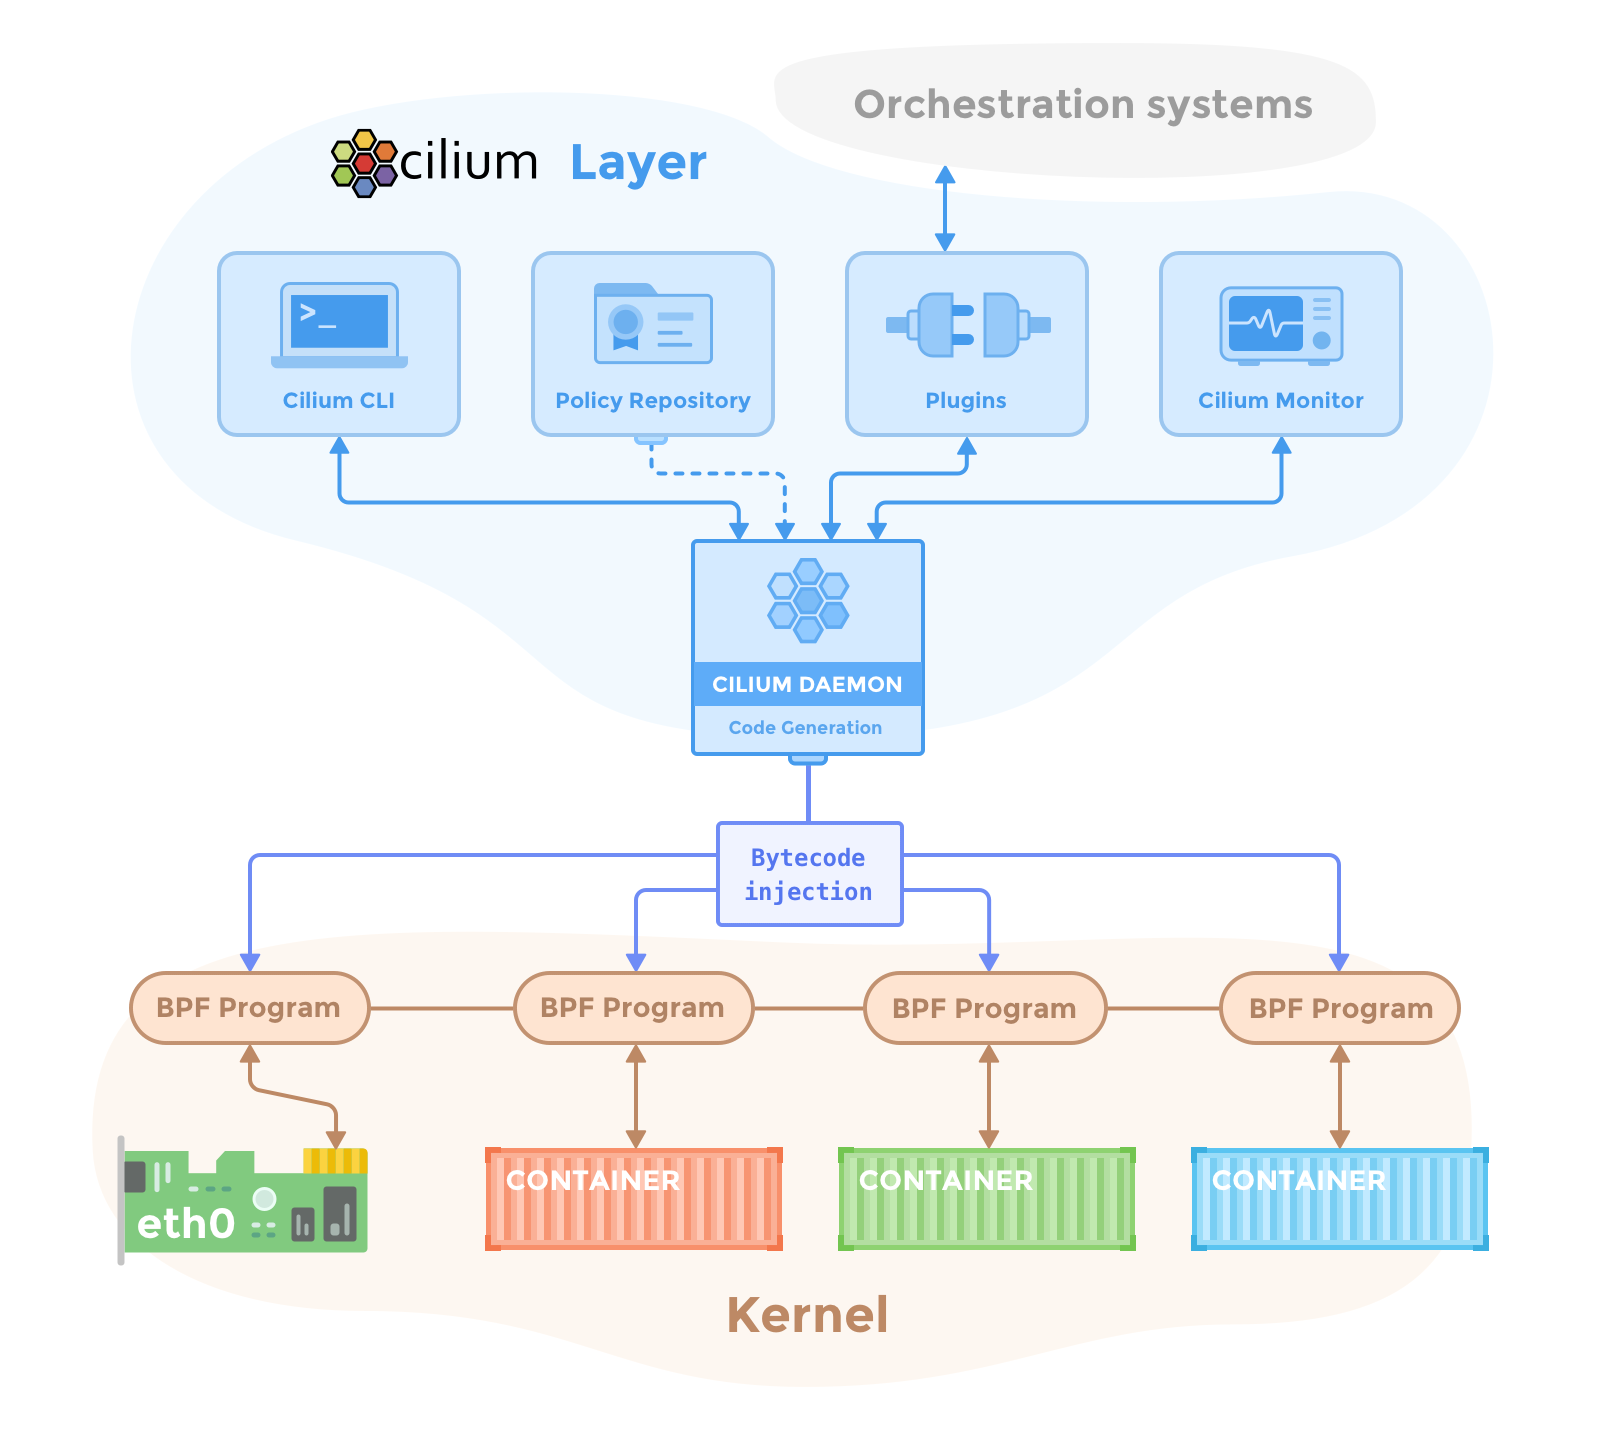
\includegraphics[width=0.8\textwidth,keepaspectratio]{cilium_architecture.png}
    \end{frame}

    \begin{frame}{ELF Templating}
        \centering
        \includesvg[width=\textwidth]{bpf-templating.svg}
    \end{frame}

    \begin{frame}{1K nodes: Scaling to 60k pods}
        \centering
        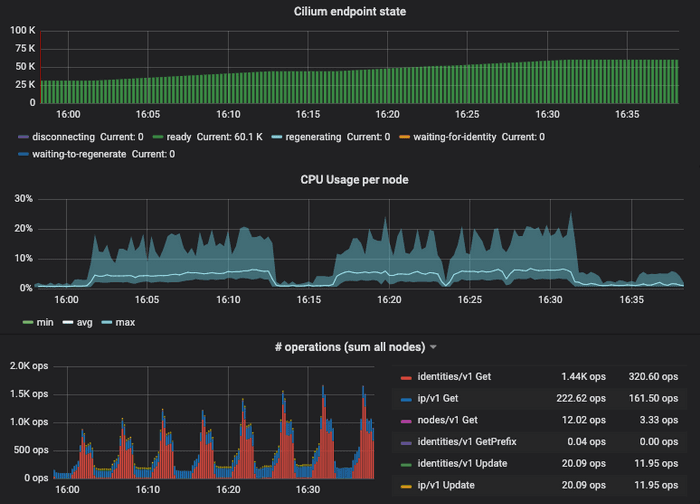
\includegraphics[width=0.8\textwidth]{scaling_to_60k_pods.png}
    \end{frame}

    \newsectionpage{Identity-based security}

    \begin{frame}{Policy model}
        \begin{itemize}
            \item Whitelist \medskip
            \pause
            \item L3 \smallskip
                \begin{itemize}
                    \item Pod labels \medskip
                    \item FQDN \medskip
                    \item Services \medskip
                \end{itemize}
            \pause
            \item L4 \medskip
            \pause
            \item L7 \smallskip
                \begin{itemize}
                    \item HTTP \medskip
                    \item DNS \medskip
                    \item Your protocol here \medskip
                \end{itemize}
        \end{itemize}
    \end{frame}

    \begin{frame}{Policy example}
        \lstinputlisting[language=yaml,%
                         showstringspaces=false,%
                         basicstyle=\footnotesize,%
                         breaklines=true]{../sw-l3-l4-policy.yaml}
        \blfootnote{\tiny \url{https://docs.cilium.io/en/stable/gettingstarted/http/}}
    \end{frame}

    \begin{frame}
        \centering
        \vfill
        \begin{figure}
            \includesvg[width=\textwidth]{identity-security.svg}
        \end{figure}
        \vfill
        \blfootnote{{\tiny Thomas Graf, {\em Cilium \& BPF - The Future of Networking and Security}, openSUSE Conference 2019}}
    \end{frame}

    \begin{frame}{... memoization something something ...}
    \end{frame}

    \newsectionpage{Proxying layer 7 requests}

    \begin{frame}{Datapath Configuration}
        \centering
        \vfill
        \begin{figure}
        \begin{overprint}
            \onslide<1>\includesvg[width=0.9\textwidth]{cilium-bpf-egress-l3.svg}
            \onslide<2>\includesvg[width=0.9\textwidth]{cilium-bpf-egress-l7.svg}
            \onslide<3>\includesvg[width=0.9\textwidth]{cilium-bpf-egress-proxy.svg}
        \end{overprint}
        \end{figure}
        \vfill
    \end{frame}

    \begin{frame}{L7 Configuration: Past}
        \centering
        \begin{overprint}
            \onslide<1>\includesvg[width=\textwidth]{bpf-proxy-nat-0.svg}
            \onslide<2>\includesvg[width=\textwidth]{bpf-proxy-nat-1.svg}
            \onslide<3>\includesvg[width=\textwidth]{bpf-proxy-nat-2.svg}
            \onslide<4>\includesvg[width=\textwidth]{bpf-proxy-nat-3.svg}
        \end{overprint}
    \end{frame}

    \begin{frame}{L7 Configuration: Present}
        \centering
        \begin{overprint}
            \onslide<1>\includesvg[width=\textwidth]{bpf-proxy-tproxy-0.svg}
            \onslide<2>\includesvg[width=\textwidth]{bpf-proxy-tproxy-1.svg}
            \onslide<3>\includesvg[width=\textwidth]{bpf-proxy-tproxy-2.svg}
            \onslide<4>\includesvg[width=\textwidth]{bpf-proxy-tproxy-3.svg}
            \onslide<5>\includesvg[width=\textwidth]{bpf-proxy-tproxy-4.svg}
        \end{overprint}
    \end{frame}

    \begin{frame}{L7 Configuration: Proposal}
        \centering
        \includesvg[width=\textwidth]{bpf-proxy-demux.svg}
    \end{frame}

    \begin{frame}[fragile]{Socket assign: Next steps \#1}
        \centering
        \begin{itemize}
            \item Resolve \verb+skb_orphan()+ issue \smallskip
            \begin{itemize}
                \item BPF progs are attached at TC ingress \medskip
                \pause
                \item Orphan invoked directly before \verb+PREROUTING+ \medskip
                \pause
                \item TC folks are already carrying hacks for this\footnotemark \medskip
                \pause
                \item Just move to \verb+____dev_forward_skb()+\footnotemark? \medskip
            \end{itemize}
            \pause
            \item Propose \verb+bpf_sk_assign()+ helper \medskip
        \end{itemize}
        \footnotetext[1]{\tiny \url{https://www.mail-archive.com/netdev@vger.kernel.org/msg303851.html}}
        \footnotetext[2]{\tiny \url{https://www.mail-archive.com/netdev@vger.kernel.org/msg304057.html}}
    \end{frame}

    \begin{frame}[fragile]{Socket assign: RFC}
        \centering
        \lstinputlisting[language=c,%
                         showstringspaces=false,%
                         basicstyle=\scriptsize,%
                         breaklines=true]{../sk-assign.c}
    \end{frame}

    \section*{}
    \begin{frame}{Thank you}
        \centering
        \vfill
        \begin{table}
            \begin{subtable}[l]{0.6\textwidth}
            \begin{tabular}{rl}
                \multicolumn{2}{l}{\textbf{More information}} \\ \\
                \includesvg[width=0.045\textwidth]{slack.svg}
                & \link{https://cilium.io/slack} \\
                \includesvg[width=0.045\textwidth]{github.svg}
                & \link{https://github.com/cilium/cilium} \\
                \includesvg[width=0.045\textwidth]{www.svg}
                & \link{https://cilium.io} \\
                \includesvg[width=0.045\textwidth]{twitter.svg}
                & \link{https://twitter.com/ciliumproject} \\
            \end{tabular}
            \end{subtable}
        %    \begin{subtable}[l]{0.45\textwidth}
        %        \textbf{More Information} \medskip
        %        \link{https://cilium.io/slack} \medskip
        %        GitHub:~\link{https://github.com/cilium/cilium} \medskip
        %        Website:~\link{https://cilium.io/} \medskip
        %        Twitter:~\link{https://twitter.com/ciliumproject}{@ciliumproject}
        %    \end{subtable}
            \begin{subtable}[r]{0.35\textwidth}
                \includesvg[width=0.9\textwidth]{cilium-gopher.svg}
            \end{subtable}
        \end{table}
        \pause
        \vfill
    \end{frame}

    \appendix
    \backupbegin
    \begin{frame}[fragile]{Socket assign: API quirks \#2}
        \centering
        \begin{itemize}
            \item Nit: Need to use \verb+sock_common+ socket lookups \medskip
            \item Add \verb+bpf_skc_lookup_udp()+ \medskip
            \item Optimization: Add lookup flags to \verb+bpf_sk*_lookup_*()+ \medskip
        \end{itemize}
    \end{frame}
    \backupend

\end{document}
